% !TeX encoding = UTF-8
% !TeX root = V30_Nonlinear.tex
% !TeX spellcheck = en_US

\section{Introduction}
Lasers have become standard equipment of many physical and chemical laboratories due to their sharp wavelength and coherence. Industrial applications, like optical disk drives and laser cutters, profit from their focused beam and the relatively high efficiency of some laser types.

While students are taught about lasers long before the advanced physics lab, understanding them doesn't mean they are able to handle them appropriately; for this reason we shall experience the occurring phenomena and difficulties first-hand.

.In the following experiment, we
\begin{itemize}
\item Measure the emitted wavelength and power of a laser diode in function of temperature and provided current
\item Construct a diode pumped Nd:YAG laser from it
\item Gauge the lifetime of the excited state with respect to spontaneous emission
\item Find the optimal wavelength to pump the Nd:YAG laser
\item Measure the output power of the (infrared) laser in function of the power of the diode laser
\item Add a nonlinear medium to double the frequency
\item Measure the output power of the new green laser mode in function of the power of the fundamental.
\end{itemize}

By trying to maximize the efficiency of our laser, we learn about adjusting lasers as well as some details about their working principle.

\newpage
\section{Theory}
Consider a system of two energy levels $E_1,~E_2$ which each can hold a large number $n_1,~n_2$ of electrons (as the Pauli theorem forbids them to be in the same quantum state, these levels stretch over numerous atoms). The energy difference $\Delta E = h \nu$ shall correspond to photons in or around the visible spectrum.

In thermodynamic equilibrium, the electrons are distributed corresponding to the Fermi-Dirac distribution, which can be approximated with the Boltzmann distribution for relatively high temperatures $T$, which includes room temperature. With $n_{tot}=n_1 + n_2$ we obtain the partition function $Z_1$ for one electron and the populations on both levels:
\begin{align}
Z_1  ~&=~ e^{-E_1/k_B T} + e^{-E_2/k_B T} \\
n_i ~&=~ n_{tot} \cdot \frac{e^{-E_i/k_B T}}{Z} \qquad i \in \{1, 2\}\\
\frac{n_2}{n_1} ~&=~ \frac{e^{-E_2/k_B T}}{e^{-E_1/k_B T}} ~=~ e^{- \Delta E/k_B T} ~<~ 1	\label{eq:pop}
\end{align}

There are three processes that transfer electron between these levels directly without involving additional energy levels:
\begin{description}
\item[Absorption] is the excitation of electrons from the lower level by absorbing a photon of the corresponding energy. The transition rate is proportional to the intensity $I$ of the light beam: $\dot n_2 = B_{12} \; n_1 \cdot I$.
\item[Stimulated emission] is the reverse process, where a resonating photon induces an electron from the upper level to emit another photon of the same energy, direction, polarization and phase. Therefore, the second photon is coherent to the original one. Again, this scales with the intensity: $\dot n_2 = -B_{21} \; n_2 \cdot I$.
\item[Spontaneous emisison] is the autonomous transition of excited electrons to the lower level , driven by the Hamiltonian principle and allowed due to a slight overlap of the wave functions corresponding to the two states. It only depends on the excited population: $\dot n_2 = -A_{21} \; n_2$.
\end{description}

Normally, these processes lead to $n_2$ being at most equal to $n_1$ for high intensities of the irradiated light, and for $I=0$ we remain in thermodynamic equilibrium with $n_2 < n_1$ for any temperature $T$  as seen in equation \eqref{eq:pop}.

By pumping electrons out of the lower level $E_1$ and to the upper level $E_2$ (by means which shall be discussed later, involving aforementioned additional energy levels), we can achieve $n_2 \gg n_1$ (population inversion) and thus prepare the system in a state where the surplus of excited electrons can be de-excited collectively via stimulated emission, creating a laser (an acronym for "light amplification by stimulated emission of radiation").

In order to create a chain reaction where electrons continuously are stimulated to emit photons, the intensity inside the active material has to be kept high. This is realized by a resonator around it reflecting most of the photons back into the laser to stimulate others. Only a (typically tiny) part of the light is sent out, so that the stimulated emission by the remaining photons suffices to sustain the lasing. For one cycle in the cavity, the amplification is called gain and the released or otherwise disappearing photons are considered losses. Only when the former outweigh the latter we have a continuous beam. In fact, many active materials have multiple transitions that could be used for a laser, and the gain/loss profile can be used to suppress all but one mode for which lasing should occur (sometimes referred to as "the winner takes it all"). The most common way to select the frequency is the resonator:
\begin{itemize}
\item Only wavelengths of which the resonator length $L$ is a multiple of can resonate in the cavity.
\item If the resonator consists of two mirrors, using a dichroic reflector as one of them will only allow a small band of wavelengths to be held back in the resonator.
\end{itemize}

\newpage
\subsection{Laser diode}
\enlargethispage{2em}
A laser diode is a p-n junction with a band gap $\Delta E$ where a voltage is applied in forward direction. Electrons flow onto the conduction band of the n-side, while they are drawn from the valence band of the p-side, which is equivalent to adding positive virtual particles $h^+$ called holes.

\begin{figure}[h]
	\centering
	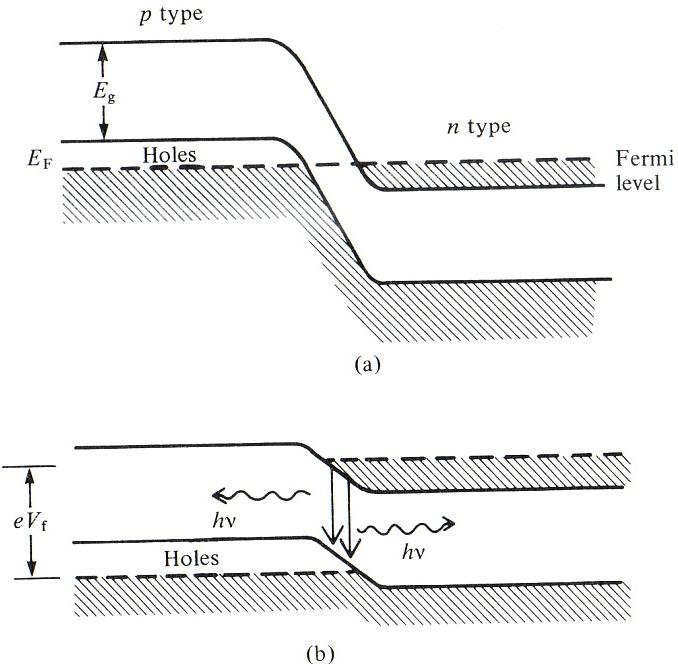
\includegraphics[width=0.6\textwidth]{diode_laser}
	\caption{Band diagram of a pn-diode: a) no current, b) current applied. \cite{lit:leicester}.}
	\label{fig:diode}
\end{figure}

As each electron hole recombination produces one photon, the possible output power is proportional to the applied injection current $I$. As we are only interested in the power $P$ of the laser beam, we first need to provide the threshold current $I_{min}$ at which the gain through stimulated emission outbalances the losses. Because the internal resonator of a diode laser is based on the cleavage planes of the crystal with about 30\% reflectivity, it requires a rather high threshold current before it actually reaches lasing.

With increasing temperature the collision rate of the electrons rises, causing electrons to disperse their energy in multiple steps and thus without emitting a photon. These additional losses lead to an increased threshold, resulting in less laser power at a given current.

Due to the fact that we have energy bands instead of levels, laser diodes emit in a considerable spectral range. Additionally, the wavelength and output power vary with both the temperature of the diode, which we will model as a linear dependency in equation \eqref{eq:lambda1}. 


\subsection{Nd:YAG laser}
The second laser used in the experiment is based on a Nd:YAG crystal (yttrium aluminium garnet doped with neodymium) which is pumped optically with the diode laser from the previous part.

For our laser, the \textsf{Nd} atoms can be approximated as a 4 level system, as displayed in figure \ref{fig:spectrum}:
\begin{itemize}
\item 1 $\rightarrow$ 4 : Absorption of red light around 805\,nm from the laser diode
\item 4 $\rightarrow$ 3 : Decay into state 3
\item 3 $\rightarrow$ 2 : Emission of infrared light at 1064\,nm
\item 2 $\rightarrow$ 1 : Decay into state 1
\end{itemize}


As the decays are nearly instantaneous, only states 1 and 3 are populated:
\begin{equation}
n_2 \approx n_4 \approx 0
\end{equation}

Levels 1 and 4 are used to optically pump electrons into state 3 and thus obtain the necessary population inversion, while the two state system for lasing consists of levels 2 and 3.

As most lasers, the one constructed in chapter \ref{sec:1064} uses a two mirrors as its resonator: One edged, one round. A pair of two planar mirrors wouldn't focus the beam back into the centre of the lasing material, while two spherical mirrors allow certain tilted beams to be in resonance, leading to transverse modes in the resonator which diminish the power available to the main mode. The compromise of a hemispherical resonator (planar mirror + spherical mirror) is easy to adjust and focus, although it doesn't suppress transverse modes as efficiently as a pure planar setup would. It is worth noting that, for any spherical mirrors, the mirror separation $L$ has to be below the curvature radius of the mirror in order to reflect the light back into the active material (stability criterion).

As the goal is to couple out a laser beam from the resonator for the transition at 1064\,\nano\metre, one of the mirrors is a dichrioc reflector which is highly reflective for a specific wavelength but nearly transparent for most others. The small fraction of the laser light passing this mirror serves as the laser beam, but over 95\% of the photons are held back.

\begin{figure}[p]
	\centering
	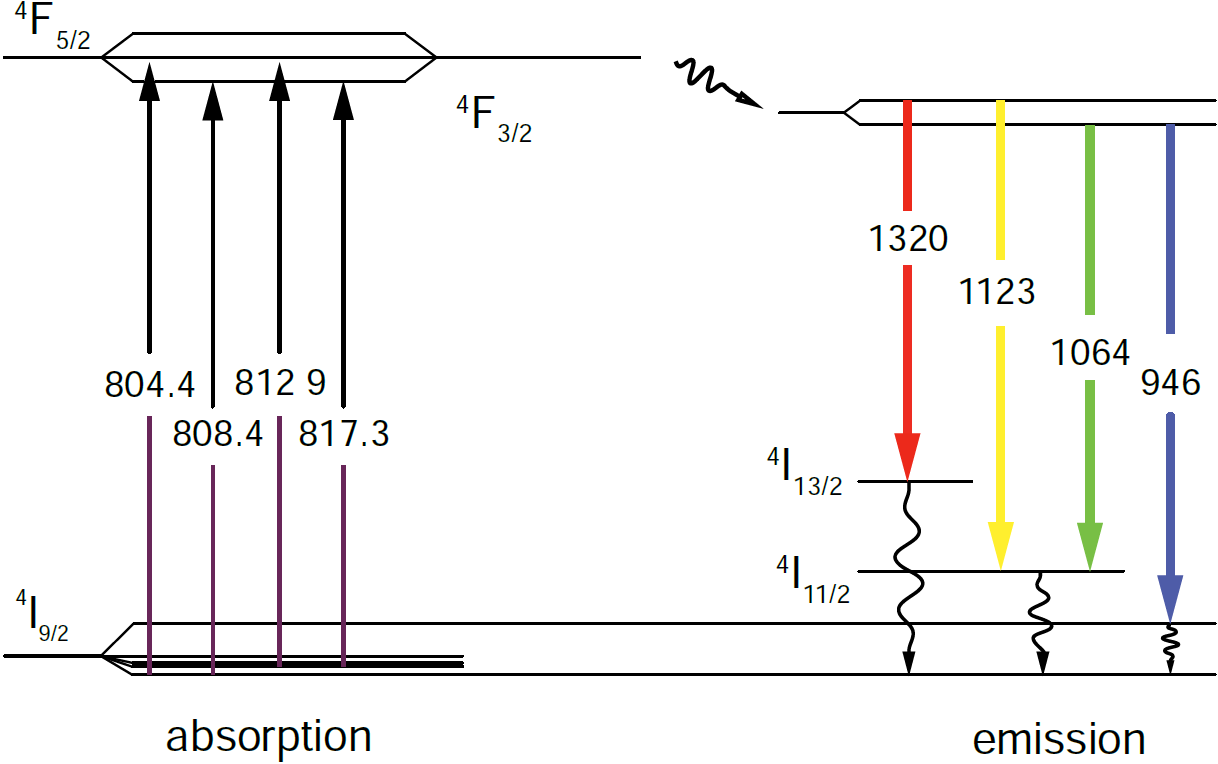
\includegraphics[width=0.9\textwidth]{spectrum.png}
	\caption{Transitions in the Nd:YAG crystal \cite{lit:leybold}.}
	Our laser is based on the absorption at 808,4\,\nano\metre{} and emission at 1064\,\nano\metre.
	\label{fig:spectrum}
\end{figure}

\begin{figure}[p]
	\centering
	\def\svgwidth{0.7\textwidth}
	\input{graphics/Nonlinear.pdf_tex}
	\caption{Nonlinear polarization deforming $\vec D$ \cite{lit:manual}.}
	\label{fig:nonlinear}
\end{figure}

\subsection{Nonlinear effect}
If a KTP crystal (Potassium titanyl phosphate, $\mathsf{K\,TiO\,PO_4}$) is inserted into the resonator of the Nd:YAG laser, the nonlinear optic properties of the crystal will enable a two photon effect where the electric field is deformed and the second harmonic of the original wave emerges. This leads to pairs of infrared photons being converted to green photons with the doubled energy (frequency doubling).

The nonlinearity is caused by the polarization of the medium showing a saturation effect and being capped for high electric fields $\vec E$ of the light beam (cp. figure \ref{fig:nonlinear}). The displacement field $\vec D$ thus is deformed relative to $\vec E$ and a Fourier transformation shows that the new wave contains a component with doubled frequency which is proportional to the square of the fundamental.

However, this process is only allowed if energy and momentum of the involved photons are conserved (or nearly conserved, due to Heisenberg's uncertainty principle).

From the energy conservation  we deduce with $E = h \nu$ that
\begin{equation}
	\nu_2 = 2 \nu_1
\end{equation}

The de Broglie wavelength can be used to write the momentum as  $\vec p = \hbar \vec k$, thus
\begin{equation}
	\vec k_2 = 2 \vec k_1
\end{equation}

With $k = \frac{2 \pi}{\lambda}$ and the dispersion relation $c = n c_0 = \lambda \nu$ we conclude that
\begin{equation}
\frac{k_2}{k_1} ~=~ 2 ~=~ \frac{n_{2\nu} \; \nu_2}{n_\nu \; \nu_1} ~=~ 2\;\frac{n_{2\nu}}{n_\nu}
\end{equation}

Thus the refraction index of the material has to be the same for both wavelengths. As most materials show normal diffraction, i.e. $n(\lambda) \searrow$ , one has to exploit that KTP is a biaxial crystal: The extrordinary index $n_{ao}(\theta)$ of refraction is larger than the ordinary index $n_o$, but depends on the angle of the beam relative to the crystal's optical axis. Thus for a certain angle $\theta$ we obtain $n_{ao, \,2\nu}(\theta) ~=~ n_{o, \,\nu}$ and the second harmonic will be clearly observable -- the original beam is infrared and therefore invisible to the human eye, only the green ray will appear.

